\subsection{Visual processing}

\paragraph{Visual processing}


In the visual system, light in the visual scene enters the eye and stimulates the cornea, the protective outer layer of the eye
\cite{KandelBook2003:26}. The light then passes through the lens, which focuses it onto the retina. The retina contains photoreceptor cells, which respond to light by transmitting electrical signals. The mentioned components of the visual system are depicted in Figure \ref{fig:receptive-field}. 

The signals from photoreceptors are passed onto so-called bipolar cells that transmit electrical (nerve) signals by inducing action potentials \cite{IzhikevichBook2004:2}. An action potential, or spike, is a nerve signal that occurs when a cell's membrane's potential suddenly rises and then rapidly falls (see Section \ref{sec:action-potential}). The spikes are propagated to target areas in the visual cortex for higher-level processing \cite{KandelBook2003:26}.

\begin{figure}[!htp]
    \centering
    \begin{tikzpicture}[
        arr/.style = { -{Stealth[ ]} },
        mainarrow/.style = {arr, draw=black, fill=black},
        shadowarrow/.style = {arr, draw=white, fill=white, very thick}
    ]
      
    \begin{scope}
        \node[anchor=south west,inner sep=0] at (0,0) {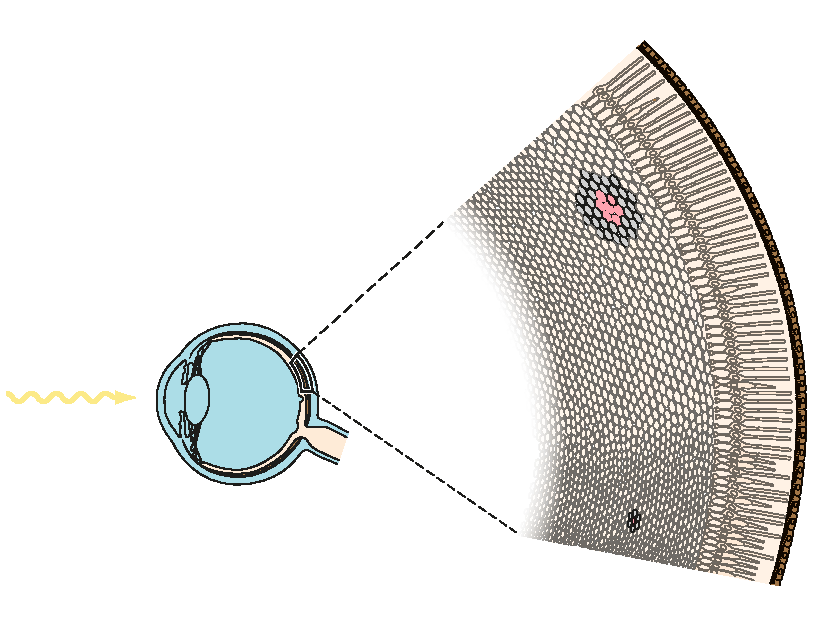
\includegraphics[width=0.8\textwidth]{assets/images/receptive-field.pdf}};
        
        % light
        \node[] (light) at (0.06\textwidth, 0.25\textwidth) {light};
        
        %cornea
        \node[] (corneatxt) at (0.15\textwidth, 0.37\textwidth) {cornea};
        \node[] (cornea) at (0.16\textwidth, 0.224\textwidth) {};
        \path [shadowarrow] (corneatxt) edge[bend right=10] node {} (cornea);
        \path [mainarrow] (corneatxt) edge[bend right=10] node {} ($ (cornea) + (-0.05, 0.2) $);
        
        %lens
        \node[] (lenstxt) at (0.2\textwidth, 0.33\textwidth) {lens};
        \node[] (lens) at (0.188\textwidth, 0.205\textwidth) {};
        \path [shadowarrow] (lenstxt) edge[bend right=7] node {} (lens);
        \path [mainarrow] (lenstxt) edge[bend right=7] node {} ($ (lens) + (-0.005, 0.2) $);
        
        % retina
        \node[] (retinatxt) at (0.33\textwidth, 0.35\textwidth) {retina};
        \node[] (retina) at (0.25\textwidth, 0.26\textwidth) {};
        \path [shadowarrow] (retinatxt) edge[bend left=7] node {} (retina);
        \path [mainarrow] (retinatxt) edge[bend left=7] node {} ($ (retina) + (0.19, 0.17) $);
        
        % fovea
        \node[] (foveatxt) at (0.4\textwidth, 0.25\textwidth) {fovea};
        \node[] (fovea) at (0.283\textwidth, 0.216\textwidth) {};
        \path [shadowarrow] (foveatxt) edge[bend left=7] node {} (fovea);
        \path [mainarrow] (foveatxt) edge[bend left=7] node {} ($ (fovea) + (0.2, 0.025) $);
        
        % receptive field
        \node[text width=0.8in] (RFperiphery) at (0.8\textwidth, 0.5\textwidth) {RF in the periphery};
        \node[text width=0.8in] (RFfovea) at (0.87\textwidth, 0.1\textwidth) {RF near the fovea};
        
    \end{scope}
\end{tikzpicture}
    \caption[Visual system and size variability of receptive fields]{Visual system and size variability of receptive fields (RF) depending on their eccentricity \cite{KandelBook2003:25}.}
    \label{fig:receptive-field}
\end{figure}

The segregation of figures from the background is an integral part of object recognition \cite{KandelBook2003:25}. It helps to separate the different objects in a scene and make them easier to identify. The visual scenes are analyzed at three levels. At the low level, discrimination on such visual attributes as local contrast, orientation, color, and movement occurs. The intermediate level is responsible for parsing an image into surfaces, their depths, shapes, and global contours. Then, finally, at the highest level of visual analysis, object identification takes place.

\paragraph{Receptive field}

The receptive field of a cell is the area on the retina that evokes a neural response to the visual stimuli (light) cast on this particular cell. Its size is measured in degrees of a visual angle, with the entire visual field nearly equal to $180^\circ$. The role of receptive fields in the visual cortex is to parse information from complex scenes into the contours of individual objects and separate them from their background.

The center of the retina, called the fovea, corresponds to the center of the gaze. The distance between the receptive field center and fovea is called eccentricity. As shown in Figure \ref{fig:receptive-field}, the size of a receptive field is smallest near the fovea and increases with eccentricity.

Receptive fields in neurons have a center-surround organization, with two distinct sub-areas: on-center and off-center (shown in pink and grey in Figure \ref{fig:receptive-field}, respectively). As illustrated in Table \ref{tab:on-off-center}, the firing response of on- and off-center cells varies depending on the location of the light in a receptive field. The regions of the spatial contrast induce a strong reaction, while little response is received from homogeneous illumination. The on- and off-center areas are mutually inhibitory, making the receptive field sensitive to borders and contours and thus enabling it to encode information about contrast.

\begin{table}[!htp]
    \centering
    \begin{tabular}{m{3cm}|c|c|c|}
\cline{3-4}
\multicolumn{2}{l|}{}                                                                  & \cellcolor{main-color}\textbf{on-center} & \cellcolor{main-color}\textbf{off-center} \\ \hline
\multicolumn{1}{|m{3cm}|}{\cellcolor{main-color}\textbf{\makecell{Light on \\ center only}}}   & \raisebox{-.5\height}{\begin{tikzpicture}
    \begin{scope}
        % to take up space
        \draw[draw=white, fill=white] (0, 0) circle (1.7cm);
        
        % off-center area
        \draw[dashed, draw=black, fill=gray-color] (0, 0) circle (1.5cm);
        % on-center area
        \draw[dashed, draw=black, fill=sec-color] (0, 0) circle (0.6cm);
        
        % light
        \draw[draw=main-color , fill=main-color] (0, 0) circle (0.3cm);
    \end{scope}
\end{tikzpicture}} & rapid firing                               & no firing                                   \\ \hline
\multicolumn{1}{|m{3cm}|}{\cellcolor{main-color}\textbf{\makecell{Light on \\ surround only}}} & \raisebox{-.5\height}{\begin{tikzpicture}
    \begin{scope}
        % to take up space
        \draw[draw=white, fill=white] (0, 0) circle (1.7cm);
        
        % off-center area
        \draw[dashed, draw=black, fill=gray-color] (0, 0) circle (1.5cm);
        % on-center area
        \draw[dashed, draw=black, fill=sec-color] (0, 0) circle (0.6cm);
        
        % light
        \draw[draw=main-color , fill=main-color] (1.05, 0) circle (0.3cm);
    \end{scope}
\end{tikzpicture}} & no firing                                  & rapid firing                                \\ \hline
\multicolumn{1}{|m{3cm}|}{\cellcolor{main-color}\textbf{\makecell{No light \\ on either}}}               & \raisebox{-.5\height}{\begin{tikzpicture}
    \begin{scope}
        % to take up space
        \draw[draw=white, fill=white] (0, 0) circle (1.7cm);
        
        % off-center area
        \draw[dashed, draw=black, fill=gray-color] (0, 0) circle (1.5cm);
        % on-center area
        \draw[dashed, draw=black, fill=sec-color] (0, 0) circle (0.6cm);
    \end{scope}
\end{tikzpicture}} & no firing                                  & no firing                                   \\ \hline
\multicolumn{1}{|m{3cm}|}{\cellcolor{main-color}\textbf{\makecell{Light on \\ both}}}          & \raisebox{-.5\height}{\begin{tikzpicture}
    \begin{scope}
        % to take up space
        \draw[draw=white, fill=white] (0, 0) circle (1.7cm);
        
        % off-center area + light
        \draw[dashed, draw=black, fill=main-color] (0, 0) circle (1.5cm);
        % on-center area + light
        \draw[dashed, draw=black, fill=main-color] (0, 0) circle (0.6cm);
    \end{scope}
\end{tikzpicture}} & mild/no firing                             & mild/no firing                              \\ \hline
\multicolumn{1}{|m{3cm}|}{\cellcolor{main-color}\textbf{\makecell{Light-dark \\ boundary}}}    & \raisebox{-.5\height}{\begin{tikzpicture}
    \begin{scope}
        % to take up space
        \draw[draw=white, fill=white] (0, 0) circle (1.7cm);
        
        % off-center area
        \draw[dashed, draw=black, fill=gray-color] (0, 0) circle (1.5cm);
        % on-center area
        \draw[dashed, draw=black, fill=sec-color] (0, 0) circle (0.6cm);
        
        % light
        \draw[draw=main-color, fill=main-color] (0.6cm, {1.5*sin(66.42)}) arc(66.42:293.58:1.5);
        
        % dashed on top
        \draw[dashed, draw=black] (0, 0) circle (0.6cm);
        \draw[dashed, draw=black] (0, 0) circle (1.5cm);
        
        
    \end{scope}
\end{tikzpicture}} & brisk firing                               & brisk firing                                \\ \hline
\end{tabular}
    \caption[Neural response depending on light location]{Response of on- and off-center neurons depending on presence and location of the light (yellow) in the receptive field \cite{KandelBook2003:25}.}
    \label{tab:on-off-center}
\end{table}

\paragraph{Grating stimuli}

Evidently, small spots of light are helpful for studying the receptive fields of single neurons. However, in order to learn about visual perception, more complex stimuli are needed \cite{KandelBook2003:26}. For instance, grating stimuli are used to investigate the perception of spatial patterns. Such stimuli are images where the luminosity varies around the mean as a sinusoidal function of space, as shown in Figure \ref{fig:grating-stimuli-examples}.
\begin{figure}[!htp]
    \centering
    \begin{subfigure}[t]{0.3\textwidth}
        \centering
        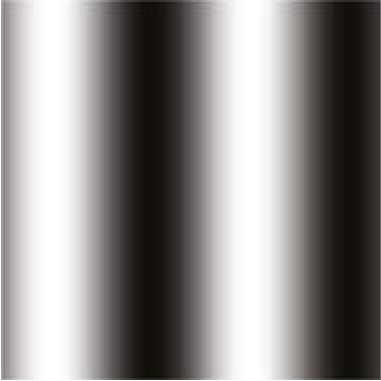
\includegraphics[width=0.65\textwidth]{assets/images/grating-stimuli/1.png}
        \caption{{Low spatial frequency.}}
    \end{subfigure}
    \hspace{0.03\textwidth}
    \begin{subfigure}[t]{0.3\textwidth}
        \centering
        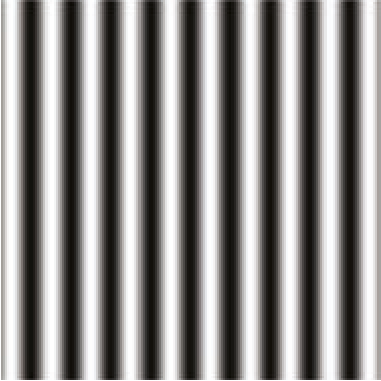
\includegraphics[width=0.65\textwidth]{assets/images/grating-stimuli/2.png}
        \caption{High spatial frequency, high contrast.}
    \end{subfigure}
    \hspace{0.03\textwidth}
    \begin{subfigure}[t]{0.3\textwidth}
        \centering
        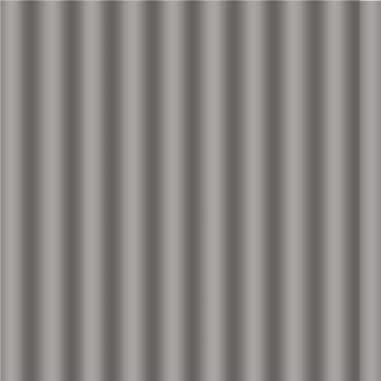
\includegraphics[width=0.65\textwidth]{assets/images/grating-stimuli/3.png}
        \caption{High spatial frequency, low contrast.}
    \end{subfigure}
    \caption[Examples of grating stimuli]{Examples of grating stimuli \cite{KandelBook2003:26}.}
    \label{fig:grating-stimuli-examples}
\end{figure}
